\documentclass[11pt]{beamer}
\usetheme{default}

\usepackage[utf8]{inputenc}
\usepackage[T1]{fontenc}
\usepackage{amsmath}
\usepackage{amsfonts}
\usepackage{amssymb}
\usepackage{graphicx}

\author{Balint Borgulya}

\title{The evolution of metabolic networks}
\subtitle{Supervisor: Bartlomiej Waclaw}
%\logo{}
%\institute{}
%\date{}
%\subject{}
%\setbeamercovered{transparent}
%\setbeamertemplate{navigation symbols}{}

\begin{document}
	\maketitle
	
	\begin{frame}
		\frametitle{Introduction}
		\begin{columns}

			\begin{column}{0.5\textwidth}
				\begin{enumerate}
					\item What is evolution? 
					\item What is a metabolic network?
					\item Why is it important?
				\end{enumerate}
			\end{column}
			\begin{column}{0.5\textwidth}
				\begin{figure}
				\centering
				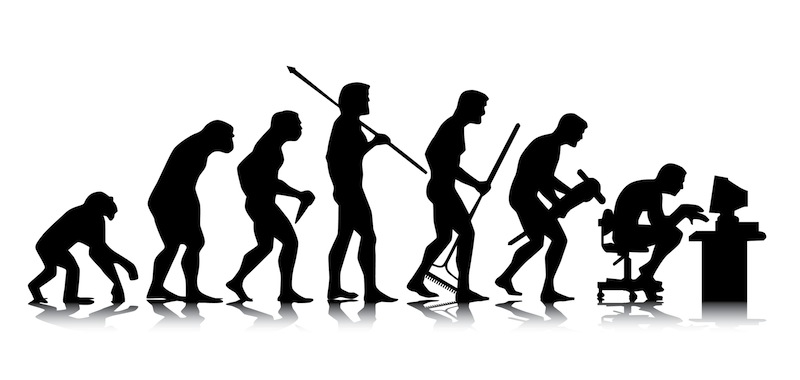
\includegraphics[width=1\linewidth]{evolution}
				\label{fig:evolution}
				\end{figure}
				
					\begin{figure}
						\centering
						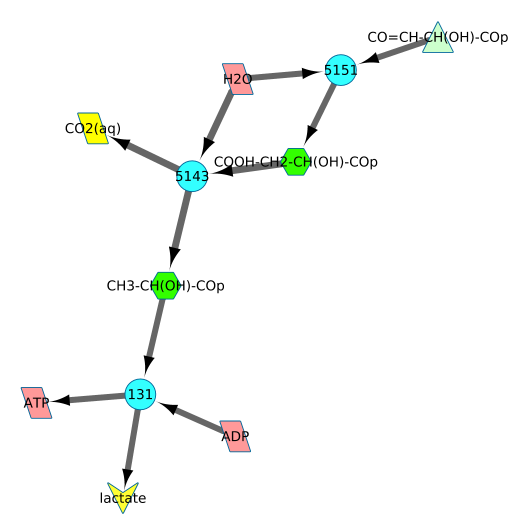
\includegraphics[width=0.9\linewidth]{initial_network}
						
					\end{figure}

			\end{column}
		
		\end{columns}
	\end{frame}
	
	\begin{frame}
		\frametitle{X-ample?}
		
		\pause
		\begin{figure}
			\centering
			
\includegraphics[width=0.36\linewidth]{walkthroughwalls_shadowcat2}
			
		\end{figure}
		
	\end{frame}
	
%	\usebackgroundtemplate{\includegraphics[width=\paperwidth]{code}}
	
	\begin{frame}
		\frametitle{The program}
		\begin{columns}
			\begin{column}{0.5\textwidth}
				\begin{figure}
					\centering
					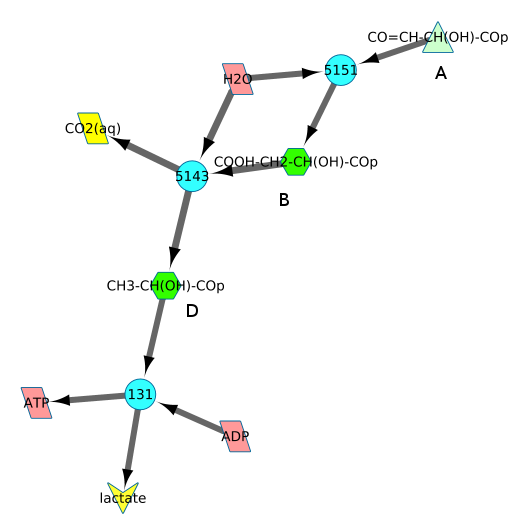
\includegraphics[width=1\linewidth]{initial_network_ABC}
					
				\end{figure}
			\end{column}
			
			\begin{column}{0.5\textwidth}
								
				\begin{figure}
					\centering
					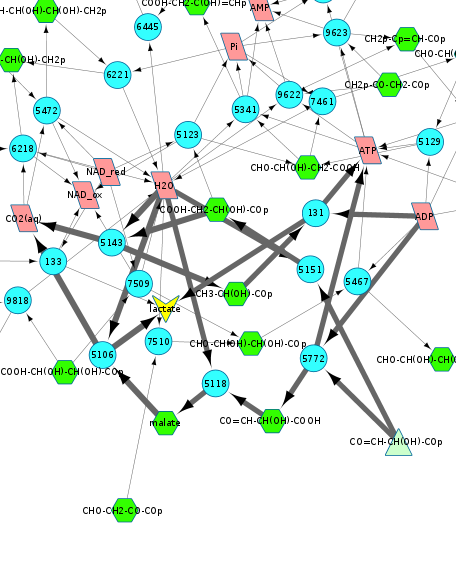
\includegraphics[width=1\linewidth]{final}
					
				\end{figure}
			\end{column}
		
		\end{columns}
		
		
	\end{frame}
	% %	\usebackgroundtemplate{\includegraphics[width=\paperwidth]{nonexistentfilename}}
	\begin{frame}
		\frametitle{Flux balance analysis}
		
		Include example matrix
		
		\begin{tabular}{|c|c|c|c|c|c|c|c|c||}
			\hline Fluxes: & 1 & 1 & 1 & 1 & 1 & 3 & -3 & \color{red} $\mathbf{1}$ \\
			\hline	Reaction: & 5151& 5143 & 131 & \multicolumn{4}{c|}{Auxiliary }& Target \\
			\hline A & -1 &  &  & +1 &  &  & &  \\ 
			\hline B & +1 & -1 &  &  &  &  & &  \\ 
			\hline D &  & +1 & -1 &  &  &  & &  \\ 
			\hline lactate &  &  & +1 &  & -1 &  & &  \\ 
			\hline H$_2$O & -1 & -1 &  &  &  &+1  & &  \\ 
			\hline CO$_2$ & +1 & +1 &  &  &  &  & +1&  \\ 
			\hline ATP &  &  & +1 &  &  &  & & -1 \\ 
			\hline ADP &  &  & -1 &  &  &  & & +1 \\ 
			\hline  
		\end{tabular} 
	\end{frame}
	
	\begin{frame}
		\frametitle{What to do next?}
		
		\begin{itemize}
			\item More complex goal functions?
			\item Dynamic changing of input/output substrate?
			\item Interaction between cells? 
		\end{itemize}
	\end{frame}
	
\end{document}